\section{Displaying Data}
When displaying data, it is important to follow the \emph{area principle}.

\begin{mdframed}
  \begin{definition}{\textbf{\underline{Area Principle:}}}
    The area principle states that the area of a graph should equal the 
    magnitude of the data it represents.
  \end{definition}
\end{mdframed}
Be careful, as many 3D graph types can violate the area principle.

\subsection{Displaying Categorical Data}
Categorical data are displayed primarily with 2 types of visual charts: Bar graphs and pie charts. It can
also be expressed with a frequency table, like the one in Figure 1.1.


\begin{figure}[h!]
  
  \centering
  \caption{An example frequency table}
  Sex of Respondents\\
  \begin{tabular}{@{}cccc@{}}
    \toprule
    Sex       & Male & Female & Total \\ \midrule
    Frequency & 13   &   10   & 23     \\ \bottomrule
  \end{tabular}
  
\end{figure}


\subsubsection{Bar Graphs}
There are many types of bar graphs. They include normal bar graphs, frequency bar graphs, and stacked
bar graphs. Below are examples of different types of bar graphs. \textbf{It is important
that the bars do not touch each other. This signifies the bars are ordered. Categorical
variables cannot be ordered in a meaningful way, so this is wrong.}
\begin{itemize}
  \item Normal Bar Graph: Displays the total number of cases in each category.
  \item Relative Frequency Bar Graph: Displays the relative frequency (percentage or decimal)
of each category. All relative frequencies add up to 100\%, or 1.
  \item Stacked Bar Graph: Shows comparisons between categories of data.
\end{itemize}

\begin{figure}[bp!]
  
  \centering
  \caption{An example of a bar graph}
  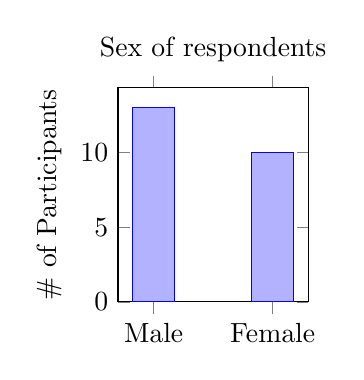
\begin{tikzpicture}
    \begin{axis}[
      title={Sex of respondents},
      ybar,
      bar width=15pt,
      enlarge x limits=0.3,
      ylabel={\# of Participants},
      symbolic x coords={Male,Female},
      xtick=data,
      ymin=0,
      width=4cm,
      height=4.3cm,
    ]
    \addplot coordinates {(Male,13) (Female,10)};
    \end{axis}
  \end{tikzpicture}

\end{figure}
\begin{figure}[bp!]

  \centering
  \caption{An example of a relative frequency bar graph}
  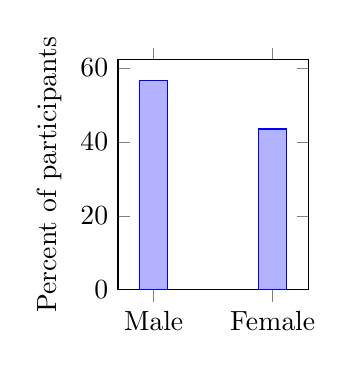
\begin{tikzpicture}
    \begin{axis}[
      ybar,
      enlarge x limits=0.3,
      ylabel={Percent of participants},
      symbolic x coords={Male,Female},
      xtick=data,
      ymin=0,
      width=4cm,
      height=4.5cm,
    ]
    \addplot coordinates {(Male,56.52) (Female,43.48)};
    \end{axis}
  \end{tikzpicture}

\end{figure}
\begin{figure}[bp!]

  \centering
  \caption{An example of a stacked bar graph}
  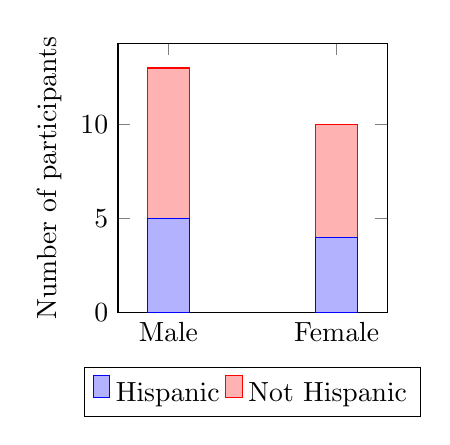
\begin{tikzpicture}
    \begin{axis}[
      ybar stacked,
      bar width=15pt,
      enlarge x limits=0.3,
      ylabel={Number of participants},
      symbolic x coords={Male,Female},
      xtick=data,
      ymin=0,
      width=5cm,
      height=5cm,
      legend style={at={(0.5,-0.20)},
      anchor=north,legend columns=-1},
    ]
    \addplot+[ybar] plot coordinates {(Male,5) (Female,4)};
    \addplot+[ybar] plot coordinates {(Male,8) (Female,6)};
    \legend{\strut Hispanic, \strut Not Hispanic}

    \end{axis}
  \end{tikzpicture}
\end{figure}
\clearpage

\subsubsection{Pie Charts}
While bar graphs are great for looking at numerical values, pie charts can 
be useful when determining the percent composition of the categories. Below
is an example of a pie chart. 

\begin{wrapfigure}{r}{0.4\textwidth}
  \caption{An example pie chart}
  \begin{small}
    \begin{tikzpicture}
    
    \pie [rotate = 45,radius=2]{56.52/Male, 43.48/Female}
    \end{tikzpicture}
  \end{small}
\end{wrapfigure}

As you can see, the pie chart does not violate the area principle. Each "slice"
of a pie chart grows in size. Polar area charts, which are similar to pie charts,
do not obey the area principle. You should also see that the sum of the relative frequencies
equals 100\%, or 1.

\subsubsection{Contingency Tables}
Similar to the stacked bar graph, these tables are used to display information
about two variables.
\begin{figure}[h!]
  
  \centering
  \caption{An example contingency table}
  Sex of Respondents\\
  \begin{tabular}{cccc}
    \hline
                                     & Male & Female & Total \\ \hline
    Hispanic                         & 5    & 4      & 9     \\ \hline
    \multicolumn{1}{l}{Not Hispanic} & 8    & 6      & 14    \\ \hline
    Total                            & 13   & 10     & 23    \\ \hline
  \end{tabular}
  
\end{figure}

The \emph{marginal frequency} of a variable is the value in the margins: the rightmost column
and the bottommost row. It can be described as $P(A)$ where $A$ is the value of the variable in
the row or column the frequency is. 

The \emph{conditional frequency} of two variables indicates the frequency
of which a variable occurs given a known value of the other. For example,
$P(Male|Hispanic)$ is $\frac{5}{9}$, which is the probability that a respondent
is male given that they are Hispanic.

\subsection{Displaying Quantitative Data}
Displaying quantitative data is a bit different from displaying categorical data.
Display methods are typically box-and-whisker plots, histograms, and stem plots.

\subsubsection{Box and Whisker Plots}


Box and Whisker plots are useful for determining these statistics:
\begin{wrapfigure}[2]{r}{0.55\textwidth}
  \caption{An example box and whisker plot}
  \begin{tikzpicture}
    \begin{axis}
      [
        ytick={1,2},
        yticklabels={1st period, 2nd period},
        xmin=50,
        xmax=100,
        ymin=0, ymax=3,
        title={AP Statistics Test Grades},
        y=1cm,
      ]
      \addplot+[
        boxplot prepared={
          median=88,
          upper quartile=92,
          lower quartile=82,
          upper whisker=95,
          lower whisker=73,
        },
      ] coordinates {};

      \addplot+[
        boxplot prepared={
          median=88,
          upper quartile=90,
          lower quartile=79,
          upper whisker=98,
          lower whisker=70
        },
      ] coordinates {(0, 55)};
    \end{axis}
    
  \end{tikzpicture}
\end{wrapfigure}

\begin{itemize}
  \item $M$/$Q_2$ (Median)
  \item $Q_1$ (First quartile)
  \item $Q_3$ (Third quartile)
  \item $minX$ (Minimum)
  \item $maxX$ (Maximum)
  \item $IQR$ (Interquartile Range)
  \item $R$ (Range)
\end{itemize}
And for determining any outliers. Outliers can be determined by individual data
points that are not included in the whisker or box.
\begin{mdframed}
  \begin{definition}{\textbf{\underline{Outlier:}}}
    As a general rule, outliers are data points that do not fall into the range
    $[Q_1-1.5*IQR,\:Q_3+1.5*IQR]$.
  \end{definition}
\end{mdframed}

\subsubsection{Histograms}
Histograms are primarily useful in order to view a distribution's shape, and any
gaps it might have.

A histogram's primary difference from a bar graph is that it is used to display 
quantitative data. This means that it has "bins", which are the bars, which touch each other.

